\documentclass[a4paper, headsepline, footheight=13.6pt]{scrartcl}
\typearea{15}
\usepackage{ae}            % nicer fonts in PDF
\usepackage{times}

\usepackage[super]{nth}
\usepackage[utf8]{inputenc} % allow utf-8 input
\usepackage[T1]{fontenc}    % use 8-bit T1 fonts
\usepackage{amsfonts}       % blackboard math symbols
\usepackage{graphicx}
\usepackage{amsmath,amssymb} % define this before the line numbering.
\usepackage{xcolor}
% \usepackage[width=122mm,left=12mm,paperwidth=146mm,height=193mm,top=12mm,paperheight=217mm]{geometry}

\usepackage{hyperref} % for clickable links in the PDF
\usepackage[all]{hypcap} % set links in figures to top
\definecolor{darkred}{rgb}{0.5,0,0}
\definecolor{darkgreen}{rgb}{0,0.5,0}
\definecolor{darkblue}{rgb}{0,0,0.5}
 
\usepackage{tabularx} % for easy text wrapping in tables

\hypersetup{linktocpage
,bookmarksnumbered=true
,colorlinks
,linkcolor=darkblue
,filecolor=darkgreen
,urlcolor=darkred
,citecolor=darkblue
,breaklinks=true
,pdfauthor={}
,pdftitle={Time evolving block decimation}
,pdfsubject={}
,raiselinks
}

% finer control of page head and foot
\usepackage[]{scrlayer-scrpage}
\pagestyle{scrheadings}
\ohead{\thepage}
\cfoot{}

\renewcommand{\equationautorefname}{Eq.}

\renewcommand{\figurename}{Figure}
\renewcommand{\figureautorefname}{Fig.}
% \renewcommand{\thefigure}{\arabic{figure}}
\renewcommand*{\captionformat}{~~\rule[-1.5pt]{0.7pt}{10pt}~~}
\setcapindent{0em}
\setkomafont{captionlabel}{\footnotesize\sffamily\bfseries}
\setkomafont{caption}{\footnotesize\sffamily}
\setkomafont{date}{\sffamily}

\usepackage{longtable}
\usepackage{multirow}
\usepackage{booktabs}  % nicer tables (\toprule, \midrule,
                       % \bottomrule)
\usepackage{colortbl}
%\usepackage{xcolor}

\usepackage{siunitx}
\sisetup{separate-uncertainty = true}

\usepackage[version=4]{mhchem}
\usepackage{textgreek}
\usepackage{braket}

\usepackage[sorting=none]{biblatex}
\addbibresource{bibliography.bib}

\title{Time evolving block decimation (TEBD)}
\date{Lent 2024}

\begin{document}
%TC:ignore

\maketitle
\newpage
\begin{abstract}
We explained and implemented the time evolving block decimation (TEBD) algorithm on a spin chain of arbitrary length and spin with periodic boundary conditions. We used imaginary time evolution with TEBD to compute the ground state of the Heisenberg XXZ model at varying $\Delta$ and obtained a mean fractional error of \qty{4e-5}{} in the ground state energy compared to the analytical solution. TEBD's linear scaling of complexity with chain length was measured and compared to the exponential scaling with chain length of exact diagonalization. Finally, we used TEBD to simulate the real time evolution of the expectation values of spin, starting with one spin anti-aligned to all others to simulate the propagation of a spin wave which was then animated. (2315 words)
\end{abstract}
%TC:endignore

\section{Introduction}
Time evolving block decimation (TEBD) is an algorithm for efficiently simulating low-energy dynamics and finding the ground state of one-dimensional quantum many-body systems with low entanglement and local interactions \cite{Vidal:2004aa}. It displays a linear scaling of computational complexity with system size, whereas alternative methods such as quantum Monte Carlo \cite{Barker:1979aa} and exact diagonalization scale exponentially with system size. TEBD works by dynamically truncating the Hilbert space to only keep the most physically relevant subspace. It relies on the matrix product state (MPS) formalism to represent the quantum state of the system, which provides an easy method to truncate the Hilbert space in a way that removes the subspace representing high entanglement states. Additionally, it relies on a Suzuki-Trotter expansion \cite{Suzuki:1990aa} to approximate the time evolution operator.

\section{Spin chains}
In this report we will consider the simulation of spin chains including finding the ground state and simulating time evolution. These are one-dimensional lattices of interacting particles where each single-particle state lies in a Hilbert space $\mathcal{H}_d$ of dimension $d$. This local dimension for a spin $s$ particle is $d=2s+1$. A state for the whole chain of $N$ sites then lies in a Hilbert space formed by the tensor product of all $N$ local Hilbert spaces: $\ket{\psi} \in \mathcal{H}^{\otimes N}_d$, which has dimension $d^N$. This exponential growth of dimension with $N$ causes exponential growth in complexity with $N$ using naive simulation methods.

To illustrate, consider a spin chain with $N=3$ and $s=\frac12$. The local dimension $d=2$, corresponding to the two local basis states $\ket{\downarrow}$ and $\ket{\uparrow}$. A basis state of the whole chain is then formed from the (ordered) tensor product of any three local basis states, for example $\ket{\uparrow\downarrow\uparrow} \equiv \ket{\uparrow} \otimes \ket{\downarrow} \otimes \ket{\uparrow}$ is a basis state of the system. This results in $d^N=2^3=8$ basis states: {$\ket{\downarrow\downarrow\downarrow}$, $\ket{\downarrow\downarrow\uparrow}$, $\ket{\downarrow\uparrow\downarrow}$, $\ket{\downarrow\uparrow\uparrow}$, $\ket{\uparrow\downarrow\downarrow}$, $\ket{\uparrow\downarrow\uparrow}$ $\ket{\uparrow\uparrow\downarrow}$, $\ket{\uparrow\uparrow\uparrow}$}.

The most natural way of describing an arbitrary state of a system of size $N$ with local dimension $d$ is then
\begin{equation} \label{eq:basis_state_sum}
    \ket{\psi} = \sum_{i_0=0}^{d-1} \cdots \sum_{i_{N-1}=0}^{d-1} c_{i_0 i_1 \cdots i_{N-1}} \ket{i_0 i_1 \cdots i_{N-1}}
\end{equation}
where $c_{i_0 i_1 \cdots i_{N-1}}$ are a set of $d^N$ complex coefficients. Thus, the state can be fully described by a vector of length $d^N$ containing these coefficients. A Hamiltonian acting on the system can then be described by a {$d^N \times d^N$} square matrix. Due to the exponential scaling, as $N$ becomes large, using standard matrix methods such as diagonalization for finding the ground state, and matrix exponentiation and multiplication for time evolution become intractable on standard computers.

\section{Quantum Heisenberg model} \label{sec:quantum_heisenberg}
The quantum Heisenberg model \cite{Heisenberg:1928aa} models magnetism as nearest-neighbour spin interactions in spin chains. Its Hamiltonian is given by
\begin{equation} \label{eq:heisenberg_hamiltonian}
    \hat{H} = \sum_{j=0}^{N-1}\left[-B\hat{S}^z_{j} - J_x \hat{S}^x_{j}\hat{S}^x_{j+1} - J_y \hat{S}^y_{j}\hat{S}^y_{j+1} - J_z \hat{S}^z_{j}\hat{S}^z_{j+1} \right]
\end{equation}
where $\hat{S}^a_j$ with is the spin operator in the $a$ direction ($a \in \{x, y, z\}$) acting only on the lattice site with index $j$; $J_a$ is the coupling constant in the $a$ direction; and $B$ is the external magnetic field. We use periodic boundary conditions such that $\hat{S}^a_{N} = \hat{S}^a_{0}$.

In order to simulate spin chains with arbitrary spin particles we have to be able to generate the spin operators $\hat{S}^a$ for any spin $s$. These can be represented as {$d \times d$} matrices with elements
\begin{align}
    \left(\mathbf{S}^x\right)_{bc} &= \frac{\hbar}{2}  \left(\delta_{b,c+1} + \delta_{b+1,c}\right) \sqrt{(s + 1)(b + c - 1) - bc} \\
    \left(\mathbf{S}^y\right)_{bc} &= \frac{i\hbar}{2} \left(\delta_{b,c+1} - \delta_{b+1,c}\right) \sqrt{(s + 1)(b + c - 1) - bc} \\
    \left(\mathbf{S}^z\right)_{bc} &= \hbar (s + 1 - b) \delta_{b,c}
\end{align}

The local Hamiltonian (i.e.\ the term inside the square brackets in \autoref{eq:heisenberg_hamiltonian}) can then be expressed as the {$d^2 \times d^2$} matrix:
\begin{equation}
    \mathbf{H}_{\text{local}} =
    -B \left(\mathbf{S}^z \otimes \mathbf{I} +
    \mathbf{I} \otimes \mathbf{S}^z\right) -
    J_x \mathbf{S}^x \otimes \mathbf{S}^x -
    J_y \mathbf{S}^y \otimes \mathbf{S}^y -
    J_z \mathbf{S}^z \otimes \mathbf{S}^z
\end{equation}
where $\otimes$ is the Kronecker product of two matrices and $\mathbf{I}$ is the {$d \times d$} identity matrix.

\section{Alternative algorithms}
\subsection{Exact diagonalization}
The ground state of the spin chain and its energy can be found by diagonalizing the Hamiltonian. Since the Hamiltonian is Hermitian and only the smallest eigenvalue and corresponding eigenstate are required, the Lanczos algorithm can be used \cite{lanczos:1950}. The Lanczos algorithm does not require forming the entire {$N^d \times N^d$} Hamiltonian matrix which would require a large amount of memory, but only requires a function that represents matrix multiplication. We can, thus, implement a function that takes as an argument the quantum state as a vector of length $d^N$ and applies the local Hamiltonian iteratively along the length of the chain, and returns the new state as another vector of length $d^N$. This significantly reduces memory usage and computational complexity.

For an {$n \times n$} matrix with mean number of non-zero elements per row $k$, the complexity of this method is $\mathcal{O}\left(kn^2\right)$. The spin chain has $n=d^N$, so exact diagonalization using the Lanczos algorithm has complexity $\mathcal{O}\left(kd^{2N}\right)$. The quantum Heisenberg model Hamiltonian has $k=2$ independent of $N$, so exact diagonalization has complexity $\mathcal{O}\left(d^{2N}\right)$. This exponential scaling with $N$ makes exact diagonalization intractable for long chains.

\subsection{Quantum Monte Carlo}
Quantum Monte Carlo (QMC) is an algorithm that simulates time evolution by solving the quantum path integral formulation numerically using Monte Carlo methods \cite{Barker:1979aa}. QMC works well for bosons but faces a numerical sign problem when dealing with fermions \cite{Dornheim:2019aa}. Additionally, its computational complexity scales with $N$ as $\mathcal{O}\left(d^N\right)$ \cite{Buividovich_2023}, which is an improvement over exact diagonalization, but still becomes intractable quickly.

\subsection{Density matrix renormalization group}
The density matrix renormalization group (DMRG) is one of the most widely used methods for simulating time evolution in quantum many-body systems \cite{Verstraete:2023aa}. DMRG could only compute the ground state when first introduced \cite{White:1992aa} but has since been extended to time-dependent DMRG (tDMRG) which uses the MPS formalism and is completely mathematically equivalent to TEBD \cite{Schollwoeck_2011}. Its computational complexity thus also scales as $\mathcal{O}(N)$.

\section{Time evolving block decimation}
The time evolving block decimation (TEBD) algorithm \cite{Vidal:2004aa} reduces the computational complexity of finding the ground state and simulating time evolution to $\mathcal{O}(N)$. It is limited to simulation of low-energy dynamics in spin chains with low entanglement and local interactions only.

\subsection{Matrix product state} \label{subsec:mps}
A key part of the TEBD algorithm is the representation of the system state as a matrix product state (MPS). The coefficients in \autoref{eq:basis_state_sum} are represented by a tensor contraction:
\begin{equation}
    c_{i_0 i_1 \ldots i_{N-1}} = 
    \Gamma^{[0]i_0}_{\alpha_{N-1}\alpha_0}
    \lambda^{[0]}_{\alpha_0}
    \Gamma^{[1]i_1}_{\alpha_0\alpha_1}
    \lambda^{[1]}_{\alpha_1}
    \Gamma^{[2]i_2}_{\alpha_1\alpha_2}
    \lambda^{[2]}_{\alpha_2}
    \cdots
    \Gamma^{[{N-2}]i_{N-2}}_{\alpha_{N-3}\alpha_{N-2}}
    \lambda^{[N-2]}_{\alpha_{N-2}}
    \Gamma^{[{N-1}]i_{N-1}}_{\alpha_{N-2}\alpha_{N-1}}
    \lambda^{[N-1]}_{\alpha_{N-1}}
    \label{eq:mps_coeffs}
\end{equation}
where $\alpha_j$ run from $0$ to $\chi-1$ and $i_j$ run from $0$ to $d-1$. $\Gamma^{[j]}$ are $N$ tensors of shape $(\chi, d, \chi)$ and $\lambda^{[j]}$ are $N$ vectors of length $\chi$ containing the Schmidt coefficients, where $\chi$ is the Schmidt rank and measures the degree of entanglement.

This report will use tensor networks to represent tensor contractions graphically. Each tensor is represented as a node and each contraction as an edge connecting two nodes. Singly connected edges represent external dimensions of the contracted tensor. For example, \autoref{eq:mps_coeffs} can be represented as the infinite tensor network in \autoref{fig:mps}, where $\lambda^{[j]}$ have been replaced with $s_j$ which are {$\chi \times \chi$} diagonal matrices with the elements of $\lambda^{[j]}$ along the diagonal and $\Gamma^{[j]}$ are labelled only by their index $j$.

\begin{figure}[htbp]
    \centering
    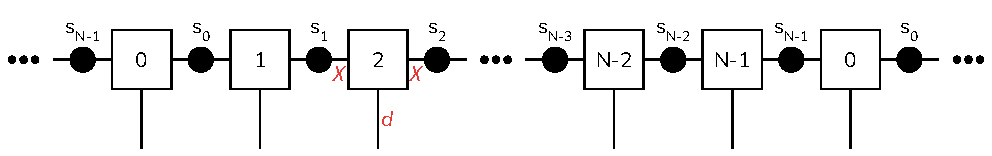
\includegraphics[width=\textwidth]{figures/mps.pdf}
    \caption{Infinite tensor network representation of a matrix product state. Square nodes with index $j$ represent the tensors $\Gamma^{[j]}$, circular nodes represent {$\chi \times \chi$} diagonal matrices $s_j$ whose diagonal elements are the elements of the vectors $\lambda^{[j]}$. The size of some dimensions is shown in red.}
    \label{fig:mps}
\end{figure}

\subsubsection{Expectation values}
To make measurements, we have to be able to calculate expectation values of operators by contracting the infinite MPS. Consider an operator $\hat{O}_{12}$ acting on sites 1 and 2. Its expectation value $\Braket{\hat{O}_{12}} = \Braket{\psi | \hat{O}_{12} | \psi}$ is the tensor contraction shown in \autoref{fig:mps_expectation}(i). Contracting an infinite MPS is not straightforward, so we define the left and right environment tensors $\sigma_j$ and $\mu_j$ which represent the contractions of the semi-infinite tensor networks in each direction starting at the bond with index $j$ (see \autoref{fig:mps_expectation}(ii)).

\begin{figure}[htbp]
    \centering
    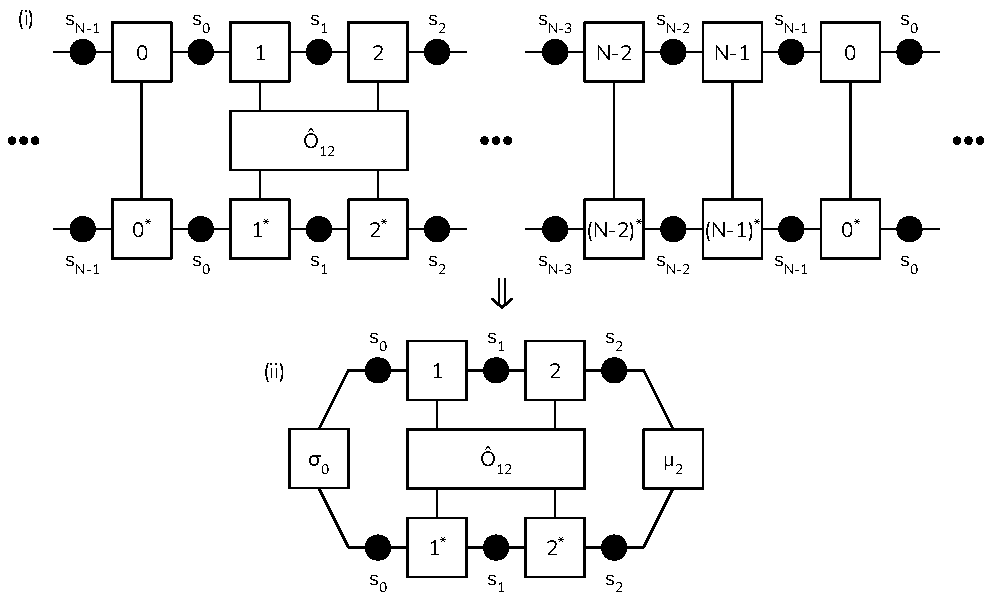
\includegraphics[width=\textwidth]{figures/mps_expectation.pdf}
    \caption{Expectation value of operator $\hat{O}_{12}$ on the infinite MPS where $^*$ represents element-wise complex conjugation. {(i):} contraction of infinite tensor network. {(ii):} semi-infinite networks replaced with environment tensors $\sigma$ and $\mu$.}
    \label{fig:mps_expectation}
\end{figure}

\begin{figure}[htbp]
    \centering
    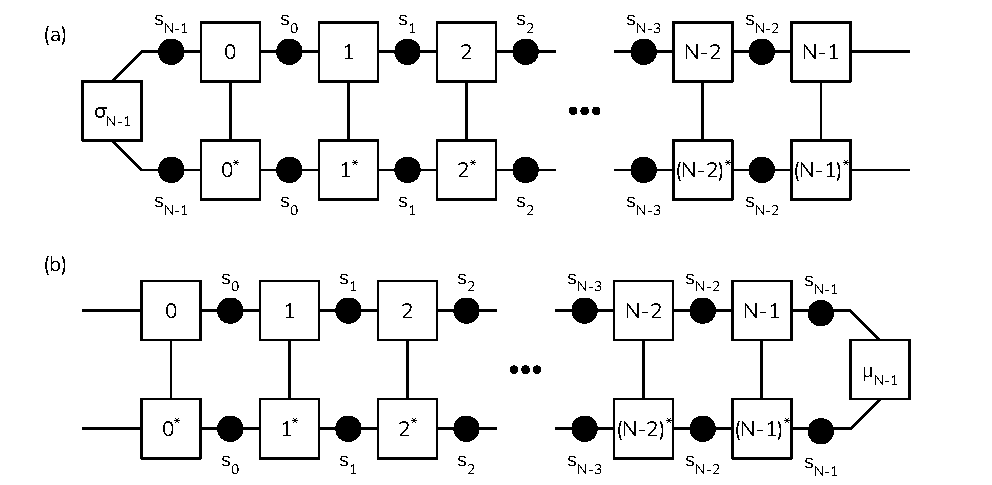
\includegraphics[width=\textwidth]{figures/transfer_operators.pdf}
    \caption{Left {(a)} and right {(b)} transfer operators.}
    \label{fig:transfer_operators}
\end{figure}

\begin{figure}[htbp]
    \centering
    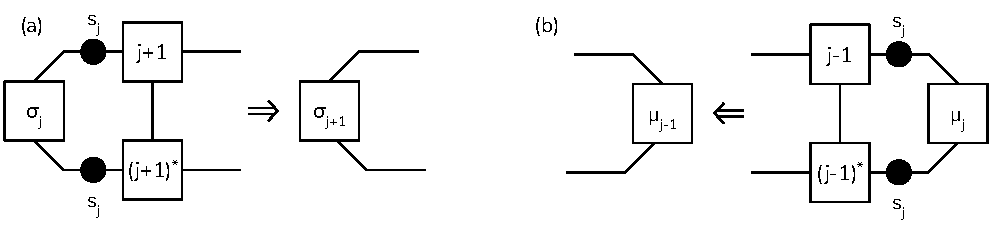
\includegraphics[width=\textwidth]{figures/environment_tensors.pdf}
    \caption{Iterative contraction for finding left environment tensors (a) and right environment tensors (b).}
    \label{fig:environment_tensors}
\end{figure}

To compute these environment tensors we define the left and right transfer operators as the contractions in \autoref{fig:transfer_operators}. The eigentensors $\sigma_{N-1}$ and $\mu_{N-1}$ of these operators with the smallest eigenvalues, which we can find using the Lanczos algorithm, are then the left and right environment tensors $\sigma_{N-1}$ and $\mu_{N-1}$. The environment tensors for all other bonds can then be found iteratively using the contractions in \autoref{fig:environment_tensors}.

\subsubsection{Canonical form}
The MPS representation is not unique since we can apply a gauge transformation as shown in \autoref{fig:canform_gauge}(a), where $\mathbf{X}$ and $\mathbf{Y}$ are absorbed into the site tensors and $\mathbf{X}^{-1}$ and $\mathbf{Y}^{-1}$ are absorbed into the weight matrix $s_j$ without changing the overall state.

We define the canonical form of an MPS as the form where all left and right environment tensors $\sigma_j$ and $\mu_j$ become identity matrices, i.e.\ $\mathbf{X}^H\sigma_j \mathbf{X} = \mathbf{I}$ and $\mathbf{Y}\mu_j \mathbf{Y}^H = \mathbf{I}$ as shown in \autoref{fig:canform_gauge}(b). Use of the canonical form ensures minimization of numerical errors accrued in tensor contractions. Thus, it is necessary to regularly canonicalize the MPS in TEBD for numerical stability. Using this form also simplifies MPS contractions and truncation of dimensions.

\begin{figure}[htbp]
    \centering
    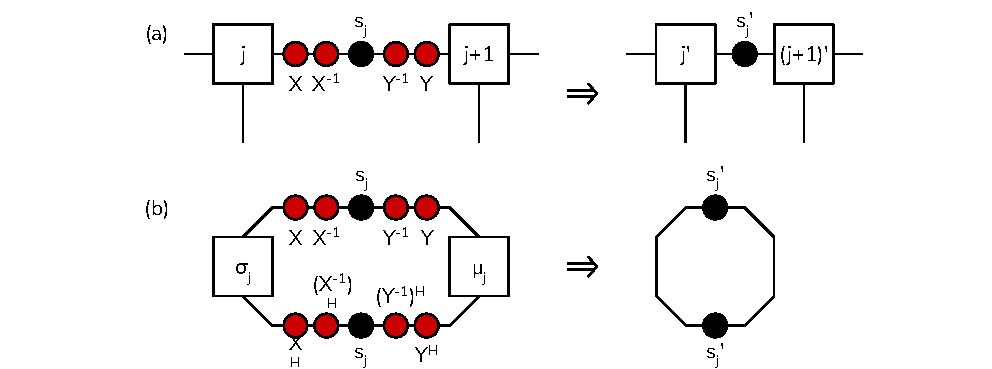
\includegraphics[width=\textwidth]{figures/canonical_form_gauge_transform.pdf}
    \caption{MPS gauge transformations, $^H$ represents the complex transpose. (a): Arbitrary gauge transformation of MPS, (b): Gauge transformation to produce canonical form}
    \label{fig:canform_gauge}
\end{figure}

The procedure to find the new weight matrix $s'$ and the gauge transformation matrices $\mathbf{X}$ and $\mathbf{Y}$ for each bond is shown in \autoref{fig:canform_process}. It can be shown that $\mathbf{X} = \mathbf{U_L}^* \frac1{\sqrt{\mathbf{D_L}}} \mathbf{U}$ and $\mathbf{Y} = \mathbf{U_R}^* \frac1{\sqrt{\mathbf{D_R}}} {\mathbf{V}^H}^T$ where $^*$ represents element-wise complex conjugation, $^T$ represents the matrix transpose, and $^H$ represents the conjugate transpose, by noting that $\mathbf{U_L}, \mathbf{U_R}, \mathbf{U}, \mathbf{V}^H$ are unitary matrices (i.e.\ $\mathbf{A}^{-1} = \mathbf{A}^H$) and $\mathbf{D_L}, \mathbf{D_R}$ are real diagonal matrices.

\begin{figure}[htbp]
    \centering
    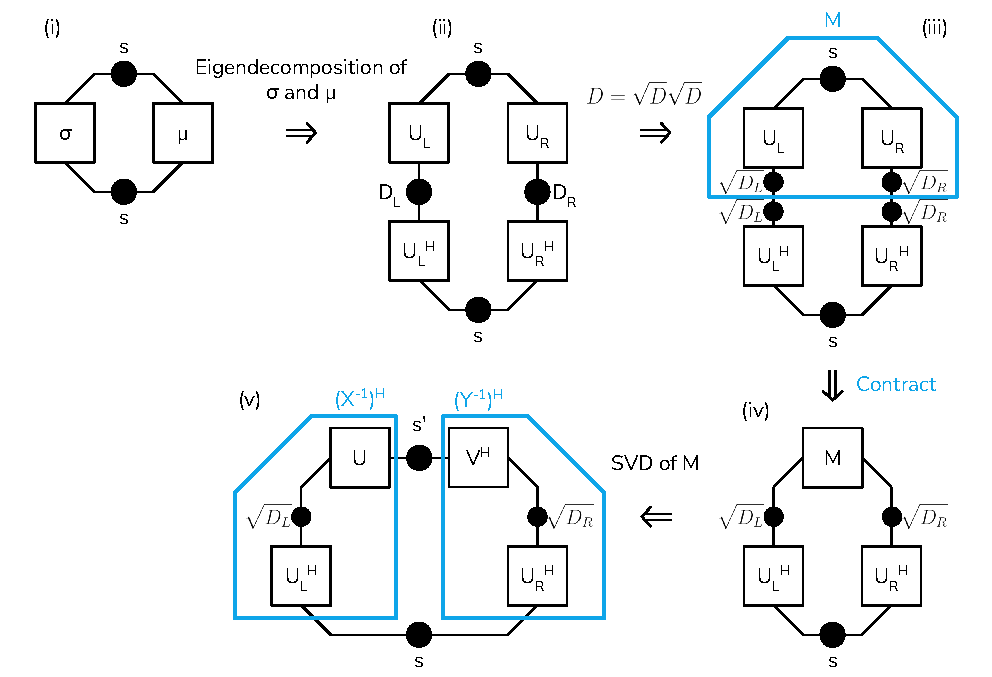
\includegraphics[width=\textwidth]{figures/canonical_form_process.pdf}
    \caption{The procedure to find the gauge transformation that results in the canonical form. SVD is the singular value decomposition.}
    \label{fig:canform_process}
\end{figure}

\subsubsection{Application of two-site gates}
If an operator acts only on two neighbouring sites it can be represented as a two-site gate which is a tensor of dimension 4 with shape $(d, d, d, d)$. The operator can then be applied to the state by contracting the gate with the local MPS and applying singular value decomposition (SVD) as shown in \autoref{fig:twosite_gate}. Another key component of TEBD is the truncation of internal dimension $\chi$ to $\chi_\epsilon$ which can be done in this step.

\begin{figure}[htbp]
    \centering
    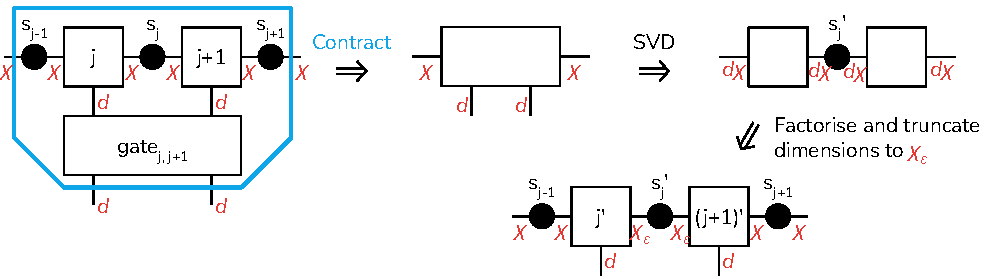
\includegraphics[width=\textwidth]{figures/two_site_gate.pdf}
    \caption{The procedure to apply a two-site gate to an MPS. SVD is the singular value decomposition.}
    \label{fig:twosite_gate}
\end{figure}

\subsection{Time evolution}
TEBD is an algorithm to efficiently evolve a state in time. The exact time evolution of a state under a time-dependent Hamiltonian $\hat{H}$ is given by the Schrödinger equation as:
\begin{equation}
    \ket{\psi(t+\mathrm{d}t)} = e^{-i\hat{H}(t)\mathrm{d}t}\ket{\psi(t)}
\end{equation}
or the discretized time version:
\begin{equation}
    \ket{\psi(t+\delta)} \approx e^{-i\hat{H}(t)\delta}\ket{\psi(t)}
\end{equation}
TEBD works on Hamiltonians that consist only of single site terms $\hat{H}_1^{[j]}$ and nearest-neighbour terms $\hat{H}_2^{[j, j+1]}$:
\begin{equation}
    \hat{H} = \sum_{j=0}^{N-1} H^{[j]} \equiv \sum_{j=0}^{N-1} \left[\hat{H}_1^{[j]} + \hat{H}_2^{[j, j+1]}\right]
\end{equation}
where we impose periodic boundary conditions such that $\hat{H}_2^{[N-1, N]} = \hat{H}_2^{[N-1, 0]}$.

In order to reduce computational complexity we would like to be able to apply each $\hat{H}_1^{[j]}$ and $\hat{H}_2^{[j, j+1]}$ separately instead of summing first, however $e^{\hat{A}+\hat{B}}=e^{\hat{A}}e^{\hat{B}}$ is only exact if $\hat{A}$ and $\hat{B}$ commute (i.e.\ $[\hat{A}, \hat{B}] = 0$) and $[\hat{H}^{[j]}, \hat{H}^{[j']}] \neq 0$ in general. Noting that $[\hat{H}^{[j]}, \hat{H}^{[j+2]}] = 0$ we can split $\hat{H}$ into an operator $\hat{F}$ acting on even $j$ sites, and an operator $\hat{G}$ acting on odd $j$ sites:
\begin{align}
    \hat{H} &\equiv \hat{F} + \hat{G} \\
    \hat{F} &\equiv \sum_{\text{even } j}^{N-2} F^{[j]} \equiv \sum_{\text{even } j}^{N-2} \left[\hat{H}_1^{[j]} + \hat{H}_2^{[j, j+1]}\right] \\
    \hat{G} &\equiv \sum_{\text{odd } j}^{N-1} G^{[j]} \equiv \sum_{\text{odd } j}^{N-1} \left[\hat{H}_1^{[j]} + \hat{H}_2^{[j, j+1]}\right]
\end{align}
assuming $N$ is even, where now $[\hat{F}^{[j]}, \hat{F}^{[j']}] = [\hat{G}^{[j]}, \hat{G}^{[j']}] = 0$, while $[\hat{F}, \hat{G}] \neq 0$ in general. The time evolution operator can then be expressed as a Suzuki-Trotter expansion of order $p$:
\begin{align}
    e^{-i\hat{H}\delta} &= e^{-i(\hat{F}+\hat{G})\delta} && \\
    &= e^{-i\hat{G}\delta} e^{-i\hat{F}\delta} + \mathcal{O}(\delta^2) & p&=1 \\
    &= e^{-i\hat{F}\delta/2} e^{-i\hat{G}\delta} e^{-i\hat{F}\delta/2} + \mathcal{O}(\delta^3) & p&=2 \\
    &\cdots &&\cdots\nonumber
\end{align}
(see \cite{Suzuki:1990aa} for higher order expansions).

We can directly apply this to evolve the MPS in time using only two-site gates. The contraction in \autoref{fig:time_evolution} shows this for the $p=1$ expansion.

\begin{figure}[htbp]
    \centering
    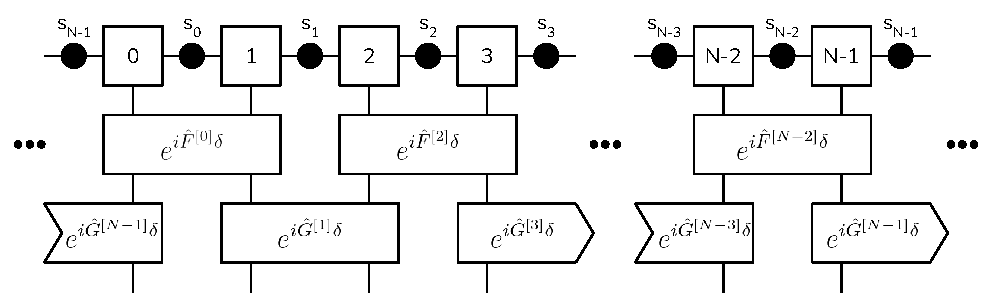
\includegraphics[width=\textwidth]{figures/time_evolution.pdf}
    \caption{MPS time evolution under first order ($p=1$) Suzuki-Trotter expansion.}
    \label{fig:time_evolution}
\end{figure}

\subsubsection{Imaginary time evolution}
If we choose $\delta$ to be imaginary negative such that $\tau=i\delta$ is real positive, we can evolve a random initial state $\ket{\psi_0}$ in imaginary time to obtain the ground state $\ket{\psi_\text{ground}}$:
\begin{equation} \label{eq:imag_time_evol}
    \ket{\psi_\text{ground}} = \lim_{\tau \rightarrow \infty} \frac{e^{-\hat{H}\tau}\ket{\psi_0}}{\left|e^{-\hat{H}\tau}\ket{\psi_0}\right|}
\end{equation}

\subsection{Truncation}
TEBD achieves $\mathcal{O}(N)$ complexity by dynamically truncating the Hilbert space $\mathcal{H}^{\otimes N}_d$.  It has been numerically observed that the Schmidt coefficients $\lambda^{[j]}_\alpha$ of the ground state and low energy excitations of a sufficiently regular one-dimensional Hamiltonian decay exponentially with $\alpha$ \cite{Vidal:2004aa}. Thus, the full state can often be very well approximated by only considering the dimensions corresponding to the $\chi_\text{trunc}$ largest Schmidt coefficients (as shown in \autoref{fig:twosite_gate}), reducing computational complexity. Since $\chi$ represents the degree of entanglement, this is equivalent to truncating the Hilbert space by removing the high-entanglement subspace.

\subsection{Errors and complexity}
The errors in TEBD come mainly from two sources \cite{Vidal:2004aa}:
\begin{enumerate}
    \item the truncation of internal dimensions
    \item the Suzuki-Trotter expansion
\end{enumerate}
Errors in the simulated state $\ket{\tilde{\psi}(t)}$ with respect to the exact state $\ket{\psi(t)}$ are measured as the fidelity error:
\begin{equation}
    \epsilon(t) = 1-\left|\Braket{\psi(t)|\tilde{\psi}(t)}\right|^2
\end{equation}

The truncation error is:
\begin{equation}
    \epsilon_1 = \sum_{\alpha = \chi_\epsilon}^{\chi-1} (\lambda_\alpha^{[j]})^2
\end{equation}
and accumulates additively as time is evolved.

The Suzuki-Trotter expansion of order $p$ neglects terms that scale as:
\begin{equation}
    \epsilon_2 \sim \delta^{2p} T^2
\end{equation}

Without truncation, the computational complexity, $T_c$, then scales as:
\begin{equation}
    T_c \sim N(d\chi)^3\left(\frac{T^{1+p}}{\epsilon^{1/2}}\right)^{1/p}
\end{equation}
which is linear in $N$ and thus a significant improvement over the exponential scaling of exact diagonalization and exact time evolution.

\section{Methods and Results} \label{sec:results}
\subsection{Imaginary time evolution} \label{subsec:imag_time_evol}
We used imaginary time evolution according to \autoref{eq:imag_time_evol} in order to find the ground state and its energy of the Heisenberg XXZ model with spins $s=\frac12$. This model is \autoref{eq:heisenberg_hamiltonian} with $J_x = J_y \neq J_z$ and $B=0$. By convention, we set $J_x = J_y = 1$ and define $J_z = \Delta$. This model has been analytically solved and has three phases \cite{Franchini_2017, Yang:1966ab, Yang:1966aa}:
\begin{itemize}
    \item $\Delta \ge 1$:
    \begin{itemize}
        \item Ferromagnetic phase
        \item Ground state: maximally polarized, i.e.\ $\Ket{\downarrow}^{\otimes N}$ and $\Ket{\uparrow}^{\otimes N}$
        \item Ground state energy per site: $E_g = -\frac{\Delta}{4}$
    \end{itemize}
    \item $ -1 < \Delta < 1$:
    \begin{itemize}
        \item Paramagnetic phase
        \item Ground state has zero magnetization
        \item Ground state energy per site:
        \begin{equation}
            E_g = \frac{\cos\mu}{4} - \frac{\sin\mu}{\mu} \int_{-\infty}^{\infty} dx \frac{\mu \sin\mu}{2\cosh(\pi x)[\cosh(2\mu x) - \cos\mu]}
        \end{equation}
        where $\Delta = -\cos\mu$ and $0 < \mu < \pi$
    \end{itemize}
    \item $ \Delta < -1$:
    \begin{itemize}
        \item Anti-ferromagnetic phase
        \item Ground state: $\Ket{\uparrow\downarrow\uparrow\downarrow\cdots}$ and $\Ket{\downarrow\uparrow\downarrow\uparrow\cdots}$
        \item Ground state energy per site:
        \begin{equation}
            E_g = \frac{\cosh\lambda}{4}-\frac{\sinh\lambda}{\lambda}\left[\frac{\lambda}{2} + 2\lambda\sum_{n=1}^{\infty}\frac{1}{1+e^{2\lambda n}}\right]
        \end{equation}
        where $\Delta = -\cosh\lambda$ and $\lambda > 0$
    \end{itemize}
\end{itemize}

For 30 evenly spaced values of $\Delta$ between $-3$ and $3$:
\begin{enumerate}
    \item A random MPS with $N=20$ and $\chi=16$ was initialized.
    \item The state was evolved by 500 time steps with $\delta=0.1$ canonicalizing the MPS every 10 time steps.
    \item The state was evolved by 2000 time steps with $\delta=0.01$ canonicalizing the MPS every 100 time steps
\end{enumerate}
The results are shown in \autoref{fig:ground_state_energy} and agree with the analytical solutions to within a mean fractional error of \qty{4e-5}{}.

\begin{figure}[htbp]
    \centering
    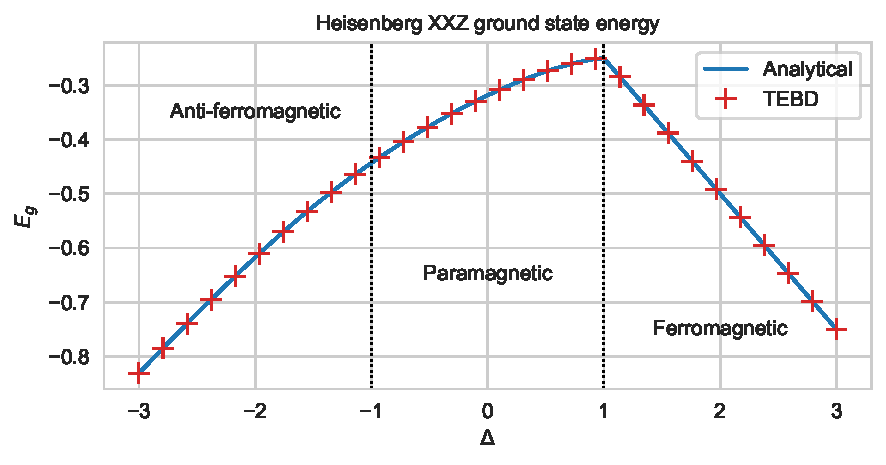
\includegraphics[width=\textwidth]{figures/ground_state_energy.pdf}
    \caption{Ground state energy of the Heisenberg XXZ model with spin $s=\frac12$ and applied field $B=0$.}
    \label{fig:ground_state_energy}
\end{figure}

\subsection{Computational complexity} \label{subsec:complexity}
We used exact diagonalization and imaginary time evolution with TEBD to solve for the ground state of the Heisenberg XX model (i.e.\ $J_x=J_y=1$, $J_z=0$) and recorded the runtime of each at varying $N$. For each $N$ we ran exact diagonalization and TEBD (500 time steps, canonicalizing every 10 time steps, $\chi_\text{trunc}=16$, $\delta=0.1$) three times on an Apple M1 Pro processor and found the mean of the runtimes. The results are shown in \autoref{fig:runtimes}. The linear scaling of TEBD runtime with $N$ can be seen clearly compared to the exponential scaling of the exact diagonalization runtime.

\begin{figure}[htbp]
    \centering
    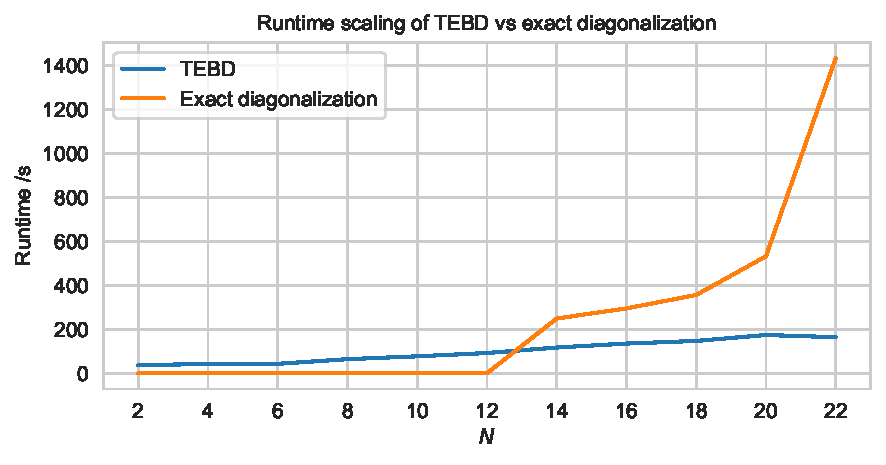
\includegraphics[width=\textwidth]{figures/runtimes.pdf}
    \caption{Mean (over three samples for each $N$) runtime of finding the ground state of the Heisenberg XX model using exact diagonalization and imaginary time evolution with TEBD (500 time steps, canonicalizing every 10 time steps, $\chi_\text{trunc}=16$, $\delta=0.1$).}
    \label{fig:runtimes}
\end{figure}

\subsection{Real time evolution} \label{subsec:real_time_evol}
We used real time evolution to simulate spin waves in the Heisenberg XXX model with $J_x=J_y=J_z=B=1$ for $s=1/2$ fermions and $s=1$ bosons:
\begin{enumerate}
    \item The MPS was prepared in the $N=30$ product state $\ket{-s}^{\otimes 14} \otimes \ket{+s} \otimes \ket{-s}^{\otimes 15}$ with $\chi=17$. 
    \item The state was evolved by 5000 time steps with $\delta=0.01$ canonicalizing the MPS and calculating the expectation values of $\hat{S}^z$ on every site every 5 time steps.
\end{enumerate}
The time evolution of these expectation values is animated in \verb|spin_half_wave.mp4| for $s=1/2$ fermions and in \verb|spin_one_wave.mp4| for $s=1$ bosons. As shown, the excited spin drops down and initiates a spin wave that propagates outwards in both directions. The bosonic spin wave propagates much faster than the fermionic spin wave. Spin waves are the basis of the field of spintronics which is analogous to electronics but uses magnons, the quanta of spin waves, instead of electrons as information carriers \cite{Hortensius:2021aa}. Simulation of spin waves is thus important to predict behaviours of such spintronic devices. Spin waves also have promising applications in quantum computing and networking \cite{Cox:2022aa}.

\section{Conclusions and outlook}
The TEBD algorithm as well as some fundamental MPS techniques were explained. We showed that imaginary time evolution with TEBD can be used to efficiently find the ground state and its energy of the Heisenberg XXZ model on a chain with $N=20$ spins, achieving a mean fractional error in the ground state energy of \qty{4e-5}{} compared to the analytical solution over a range of $\Delta$. The linear scaling of TEBD runtime with $N$ compared to the exponential scaling of exact diagonalization runtime with $N$ was measured and shown. We showed how real time evolution with TEBD can be used to efficiently simulate the propagation of spin waves in fermionic and bosonic chains.

It would be interesting to investigate the impact of using a higher order Suzuki-Trotter expansion. Additionally, It would be interesting to apply TEBD to a wider range of Hamiltonians, including time-dependent Hamiltonians and those whose ground state cannot be found analytically. Furthermore, it would be interesting to consider next-nearest-neighbour or further interactions, which would require the use of swap gates. Since only very few physically relevant systems are one-dimensional it would be interesting to extend this simulation method to higher dimensions by replacing the MPS with a projected entangled pair state \cite{Verstraete:2004cf}.

%TC:ignore
\newpage
\appendix
\section{Code structure}
\verb|mps.py| contains functions to generate and manipulate an infinite MPS, most of which correspond to the subsubsections of \autoref{subsec:mps}. \verb|tebd.py| contains functions for performing the TEBD algorithm as well as a function to create spin operator matrices for arbitrary spins as described in \autoref{sec:quantum_heisenberg}. Each subsection of \autoref{sec:results} has a corresponding Jupyter notebook that produces the results mentioned/shown there: \verb|ground_state.ipynb| contains the code for \autoref{subsec:imag_time_evol}, \verb|runtimes.ipynb| contains the code for \autoref{subsec:complexity}, \verb|spin_wave.ipynb| contains the code for \autoref{subsec:real_time_evol} and generates the animations \verb|spin_half_wave.mp4| and \verb|spin_one_wave.mp4|.

\section{Acknowledgements}
The TEBD algorithm was first proposed by Vidal \cite{Vidal:2004aa}, and many of the mathematical expressions in this report have been adapted from the original paper.

Much of the code, explanations, and diagrams has been adapted from \cite{tensorsnet} which has an implementation and explanations of TEBD on a spin chain with $N=2$. This work is thus mostly a generalization of that work to arbitrary $N$ along with some demonstrations of TEBD.

\clearpage
\newpage
\begin{flushleft}
\printbibliography
\end{flushleft}
%TC:endignore
\end{document}